\section{Research Questions}
Due to previous work not focusing on the role of symmetry groups in perception, we sought to design an experiment that tested which types of symmetry are easily perceived by humans. We also wanted to compare multiple theories of symmetry perception. In order to do this, we designed a task requiring people to differentiate wallpaper groups. Our research questions can be summarized as:

\begin{enumerate}
\item {\textbf{\textit{Can people naively distinguish among the wallpaper groups?}} In other words, without using any knowledge of symmetry, are they still able to see the differences? If the answer is yes, then we can expect that, at the very least, more features than reflection play a role in symmetry perception. Further, if people are very good at telling apart the wallpaper groups, then it is possible that group-theoretic symmetry actually plays a role in perception. This integrates well with a computational cognition paradigm.}
\item {\textbf{\textit{What features of symmetry drive the perception of symmetry?}} The presumption of previous studies is that reflection is the most important in perception, while Clarke's study claimed it was rotation. However, to the best of our knowledge, this is the first study to systematically isolate various symmetries. We will additionally investigate the role of the \textit{tile shape}}.
\end{enumerate}

\begin{figure}[!ht]
\centering
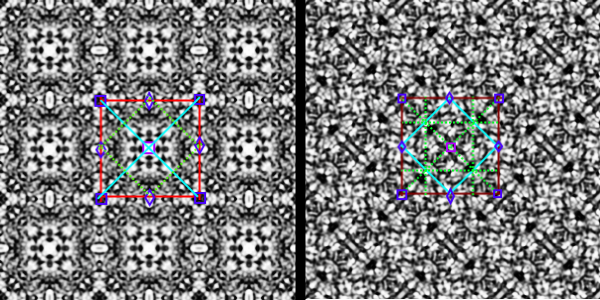
\includegraphics[width=0.9\columnwidth]{ann_images}
\caption{On the left is P4M, on the right is P4G. In each, one tile is marked with its symmetries. Notice that P4M has reflection axes on its tile border, whereas P4G does not.}
\label{fig:P4GvP4M}
\end{figure}

\begin{figure}[!ht]
\centering
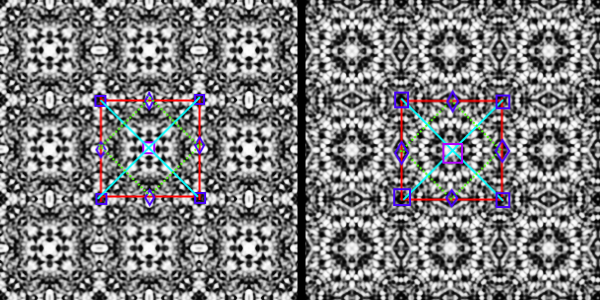
\includegraphics[width=0.9\columnwidth]{ann_images_same}
\caption{Both images are of the P4M group. Even though their appearance is quite different, they have the same symmetries in every single tile. }
\label{P4MvP4M}
\end{figure}